\documentclass[pdf,9pt,xcolor=dvipsnames,hide notes]{beamer}
\usetheme{Rochester}
%\usecolortheme{beaver}
\usepackage{verbatim}
\usefonttheme{serif}     % Font theme: serif
\usepackage{ccfonts}     % Font family: Concrete Math
\usepackage[T1]{fontenc}
\usepackage{lmodern}
\usepackage{caption}
\usepackage[caption=false]{subfig}
\usepackage{tabularx}
\usepackage{booktabs}
\usepackage{pdfpages}
\usepackage{graphicx}  
\DeclareCaptionLabelSeparator{horse}{:\quad} % change according to your needs
\captionsetup{
	labelsep = horse,
	figureposition = bottom % proper spacing between figure and caption
}
\usepackage{graphicx,amsfonts,booktabs,hyperref,subfig,amssymb,amsmath,amsthm,tabularx,multirow,enumerate}
%\usepackage{parskip}
%\setlength{\parindent}{10pt}
\usepackage{ragged2e,tikz,color,colortbl}
\usepackage[first=0,last=9]{lcg}

\DeclareMathOperator{\Ima}{Im}

% Real Number
\newcommand{\R}{\mathbb R}
% natural numbers
\newcommand{\Nat}{\mathbb N}
% complex numbers
\newcommand{\C}{\mathbb C}
\newcommand{\E}{\mathbb{E}}
\newcommand{\Var}{\mathrm{Var}}
\newcommand{\Cov}{\mathrm{Cov}}
\newcommand{\Corr}{\mathrm{Corr}}
\newcommand{\Expect}{{\rm I\kern-.3em E}}

\setbeamertemplate{theorems}[numbered]

\setbeamertemplate{caption}[numbered]
\setbeamercolor{postit}{use=structure,fg=black,bg=structure!13!white}
\newcommand{\otoprule}{\midrule[\heavyrulewidth]}
\makeatletter
\newenvironment{withoutheadline}{
	\setbeamertemplate{headline}[default]
	\def\beamer@entrycode{\vspace*{-\headheight}}
}{}
\makeatother
\title[PPGE/UFRGS]{Performance of Pairs Trading on the S\&P 500 using Distance and Mixed Copula models }
%\subtitle{}
\author[Fernando A. Boeira Sabino da Silva]{Fernando A. Boeira Sabino da Silva\inst{1}}
\author[Flavio A. Ziegelmann]{Fernando A. Boeira Sabino da Silva\inst{1,2}, Flavio A. Ziegelmann\inst{1,2}}
\author[Joao F. Caldeira]{Fernando A. Boeira Sabino da Silva\inst{1}, Flavio A. Ziegelmann\inst{1,2}, Joao F. Caldeira\inst{2}}
\institute[Department of Statistics/UFRGS, PPGE/UFRGS]{\inst{1} Department of Statistics/UFRGS, \inst{2} PPGE/UFRGS}
%\date{\today} % (optional)
\date{} % (optional)

\hypersetup{
    pdftitle={TITLE},
    pdfauthor={AUTHOR},
    pdfsubject={SUBJECT},
    pdfkeywords={KEYWORD} {KEYWORD} {KEYWORD},
    colorlinks=true,
    linkcolor=blue,
    citecolor=blue,
    filecolor=magenta,
    urlcolor=blue
    }
\usepackage{threeparttable}
\usepackage{pdfpages}  


\begin{document}
	\justifying
	
	\frame{\titlepage}
	
	%\frame{\frametitle{Table of contents}\tableofcontents}
	
	\begin{frame}
		\frametitle{Two-Dimensional Pairs Trading}
		
		\begin{figure}[htbp]
			\centering
			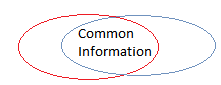
\includegraphics[scale=0.5]{fig1.png}
			\label{fig:fig1}
		\end{figure}
		
		\begin{figure}[htbp]
			\centering
			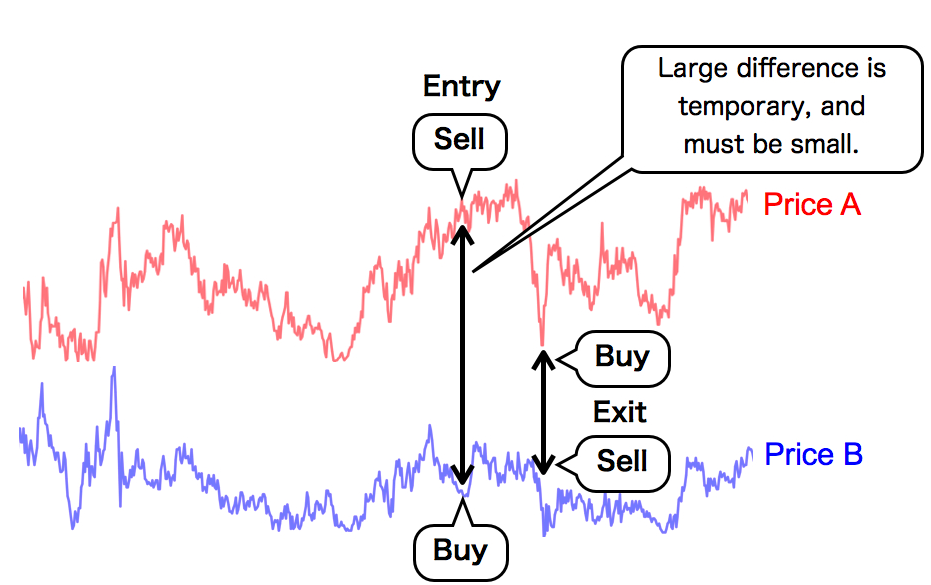
\includegraphics[scale=0.38]{fig2.png}
			\label{fig:fig2}
		\end{figure}
		
	\end{frame}
	
	\section{Pairs Trading}
	
	\begin{frame}[label=frame1]
		\frametitle{Introduction and Motivation}
		
		\begin{itemize}
			\justifying
			
			\item Pairs trading is a statistical arbitrage strategy that involves the simultaneous long/short of two
			relatively mispriced stocks which have strong historical co-movements.
			
			\vspace{0.3cm}
			
			\item The most popular strategy is known as distance method (see \textcolor{blue}{Gatev \emph{et al}}., \textcolor{blue}{2006}). 
			
		    \vspace{0.3cm}
			
			\item The distance strategy (\textcolor{blue}{Gatev \emph{et al}}.), \textcolor{blue}{2006} uses the distance between normalized prices to capture the degree of mispricing stocks. According to \textcolor{blue}{Xie \emph{et al}}., \textcolor{blue}{2014} the distance method has a multivariate normal nature since it assumes a symmetric distribution of the spread between normalized prices of the stocks within a pair and it uses a single distance measure, which can be seen as an alternative measurement of the linear association, to describe the relationship between two stocks.
			
		\end{itemize}	
	\end{frame}
	
	
	
	\begin{frame}[label=frame1c]
		\frametitle{Introduction and Motivation}
		
		\begin{itemize}
			\justifying
			
			\item Linear correlation fully describes the dependence between securities if the series have joint normal distribution. 
			
			\vspace{0.3cm}
			
			\item   However, a main feature of joint distributions characterized by tail dependence is the presence of heavy and possibly asymmetric tails. Therefore, a single distance measure may fail to catch the dynamics of the spread between a pair of securities, and thus initiate and close the trades at non-optimal positions.
			
			\vspace{0.3cm}
			
			\item \textcolor{blue}{Lie and Wu}., \textcolor{blue}{2013} proposed a pairs trading strategy based on 2-dimensional copulas to overcome the limitations of the distance method.
			
			\vspace{0.3cm}
			
%			\item 	Copulas are able to model better the empirically verified regularities normally attributed to multivariate financial returns.
%			
		\end{itemize}
		%\begin{flushright}
		%\hyperlink{counterexample}{\beamerreturnbutton{Counterexample}}
		%\end{flushright}
		
	\end{frame}
	
%	\begin{frame}[label=frame1d]
%		\frametitle{Introduction and Motivation}
%		
%		\begin{itemize}
%			\justifying
%			
%			\vspace{0.3cm}
%			
%			\item \textcolor{blue}{Lie and Wu}., \textcolor{blue}{2013} proposed a pairs trading strategy based on 2-dimensional copulas to overcome the limitations of the distance method.
%			
%%			\item 	Copulas are able to model better the empirically verified regularities normally attributed to multivariate financial returns.
%			
%		\end{itemize}
%		%\begin{flushright}
%		%\hyperlink{counterexample}{\beamerreturnbutton{Counterexample}}
%		%\end{flushright}
%		
%	\end{frame}

\begin{frame}[label=frame2]
\frametitle{Goals}

%\definecolor{bluegreen}{rgb}{0.0, 0.87, 0.87}
%\definecolor{amber}{rgb}{1.0, 0.75, 0.0}
%\definecolor{celadon}{rgb}{0.67, 0.88, 0.69}
%\definecolor{citrine}{rgb}{0.89, 0.82, 0.04}
%\definecolor{corn}{rgb}{0.98, 0.93, 0.36}
%\definecolor{darkorange}{rgb}{1.0, 0.55, 0.0}
%\definecolor{deepsaffron}{rgb}{1.0, 0.6, 0.2}
%\rowcolor{bluegreen}
%\rowcolor{amber}
%\rowcolor{celadon}
%\rowcolor{citrine}
%\rowcolor{corn}
%\rowcolor{darkorange}
%\rowcolor{deepsaffron}
%
%\begin{table}[ht]
%	\centering
%	\begin{tabular}{c|ccccccc}
%		\hline
%		\rowcolor{corn}
%		Strategy & Associations & Required Marginal \\
%		\rowcolor{corn}
%		& Captured & Distributions \\
%		\hline
%		Distance& Linear & Gaussian \\
%		Copula& Linear and Nonlinear & No assumption \\
%		\hline
%	\end{tabular}
%\end{table}

\begin{enumerate}[(1)]
\justifying

\item Conduct an empirical investigation to understand any differences in performances of the distance and copula strategies. We want to assess if a more sophisticated approach than the distance method can take advantage of any market frictions/anomalies.

\vspace{0.3cm}

\item Investigate how trading costs and different measures for pairs selection affect the profitability of these strategies.

\vspace{0.3cm}

\item Investigate the sensitivity of copula's method to different opening threshols.

\vspace{0.3cm}

\item Find if pairs trading profitability is associated to exposure to different systematic risk factors.

\end{enumerate}

\end{frame}

\subsection{Copula}
\begin{frame}[label=frame4]
	\frametitle{Copula}
	
	\begin{theorem}
		(Sklar's Theorem) Let $X_{1},...,X_{d}$ be random variables with
		distribution functions $F_{1},...,F_{d}$, respectively. Then, there exists
		an d-copula C such that,
		\begin{equation}
		F\left( x_{1},...,x_{d}\right) =C\left( F_{1}\left( x_{1}\right)
		,...,F_{d}\left( x_{d}\right) \right) ,  \label{2}
		\end{equation}
	\end{theorem}
	for all $\mathbf{x}=\left( x_{1},...,x_{d}\right) \in \mathbb{R}^{d}$.
	
	%	\item If the marginals $F_{1},...,F_{d}$ are all continuous, $C$ is
	%	unique. Otherwise $C$ is uniquely determined on $\Ima F_{1}\times ...\times \Ima %
	%	F_{d}$.
	
	\vspace{0.3cm}
	
	\begin{itemize}
		\justifying
		
		\item Assuming that $F\left( \cdot \right) $ and $C\left( \cdot
		\right) $ are differentiable, by $\left( \ref{2}\right)$ we have
		
	\end{itemize}
	
	\begin{eqnarray}
	\frac{\partial ^{d}F\left( x_{1},...,x_{d}\right) }{\partial
		x_{1}...\partial x_{d}} &\equiv &f\left( x_{1},...,x_{d}\right) =\frac{
		\partial ^{d}C\left( F_{1}\left( x_{1}\right) ,...,F_{d}\left( x_{d}\right)
		\right) }{\partial x_{1}...\partial x_{d}} \\
	&=&c\left( u_{1},...,u_{d}\right) \prod_{i=1}^{d}f_{i}\left( x_{i}\right),
	\label{23}
	\end{eqnarray}%
	where $u_{i}$=$F_{i}\left( x_{i}\right) $, $i=1,...,d$.
	
	%\item Sklar's theorem states that any multivariate joint distribution can be written in terms of their univariate marginal distribution function and the dependence structure between the variables.
	
	
\end{frame}

\begin{frame}[label=frame4b]
	\frametitle{Copula}
	
	\begin{itemize}
	\justifying
		
		\item Sklar's theorem states that any multivariate joint distribution can be written in terms of their univariate marginal distribution function and the dependence structure (represented in $C$) between the variables.
		
		\vspace{0.3cm}
		
%		\item In other words, Copulas are functions that connect a multivariate distribution function and their marginal distributions. 
		
		\item Copulas accommodate various forms of dependence through suitable choice of the copula ``correlation matrix'' since they conveniently se \linebreak parate marginals from dependence component.
		
		\vspace{0.3cm}
		
%		\definecolor{bluegreen}{rgb}{0.0, 0.87, 0.87}
%		\definecolor{amber}{rgb}{1.0, 0.75, 0.0}
%		\definecolor{celadon}{rgb}{0.67, 0.88, 0.69}
%		\definecolor{citrine}{rgb}{0.89, 0.82, 0.04}
		\definecolor{corn}{rgb}{0.98, 0.93, 0.36}
%		\definecolor{darkorange}{rgb}{1.0, 0.55, 0.0}
%		\definecolor{deepsaffron}{rgb}{1.0, 0.6, 0.2}
%		\rowcolor{bluegreen}
%		\rowcolor{amber}
%		\rowcolor{celadon}
%		\rowcolor{citrine}
%		\rowcolor{corn}
%		\rowcolor{darkorange}
%		\rowcolor{deepsaffron}
		
		\begin{table}[ht]
			\centering
			\begin{tabular}{c|ccccccc}
				\hline
				\rowcolor{corn}
				Strategy & Associations & Required Marginal \\
				\rowcolor{corn}
				& Captured & Distributions \\
				\hline
				Distance& Linear & Gaussian \\
				Copula& Linear and Nonlinear & No assumption \\
				\hline
			\end{tabular}
		\end{table}
		
%		\item No assumption on the joint behavior of the marginals is required, which provides a great deal of flexibility in modeling joint distributions.

		\vspace{0.3cm}
%		
%		\item Copula separates the estimations of individual marginal distributions and joint distribution into two different procedures, which makes it a powerful tool as it eliminates the need to imply normal distribution of stock returns.
		
		%		\item We can interpret the copula as the adjustment that
		%		we need to make to convert the independence probability density function
		%		into the multivariate density function. 
		%		
		%		\vspace{0.3cm}
		%	
		\vspace{0.3cm}
			
		\item From a modelling perspective, Sklar's Theorem allow us to estimate the multivariate distribution in two parts: (i) finding the marginal distributions; (ii) finding the dependency between the filtered data from (i).
		
	\end{itemize}
\end{frame}

%\begin{frame}[label=frame4c2]
%	\frametitle{Copula}
%	
%	\begin{itemize}
%		\justifying

%		\item From a modelling perspective, Sklar's Theorem allow us to separate the
%		modeling of the marginals $F_{i}\left( x_{i}\right) $ from the dependence
%		structure, represented in $C$.
%		
%		\vspace{0.3cm}

%		\item The copula probability density function
%		
%	
%		\begin{equation}
%		c\left( u_{1},...,u_{n}\right) =\frac{f\left( x_{1},...,x_{n}\right) }{
%			\prod_{i=1}^{n}f_{i}\left( x_{i}\right) }  \label{24}
%		\end{equation}%
%		
%
%	is the ratio of the joint probability function to what it would have been under independence. 
%	
%	\vspace{0.3cm}
%	
%	\item We can interpret the copula as the adjustment that
%		we need to make to convert the independence probability density function
%		into the multivariate density function. 
%		
%		\vspace{0.3cm}
%		
%		\item We can estimate
%		the multivariate distribution in two parts: (i) finding the marginal
%		distributions; (ii) finding the dependency between the filtered data from
%		(i).
%		\end{itemize}
%\end{frame}

\section{Data}
\begin{frame}[label=frame2b]
	\frametitle{Data}
		\begin{itemize}
		\justifying
		
		\item 	Daily data of adjusted closing prices of all shares that belongs to the S\&P500 market index from July 2nd, 1990 to December 31st, 2015. We obtain the adjusted closing prices from Bloomberg and the returns on the Fama and French factors from French's website. 
		
		\vspace{0.3cm}
		
		\item The data set sample period is made up of 6,426 days and includes a total of 1100 stocks over all periods. Only stocks that are listed during the formation period are included in the analysis, \emph{i.e.}, around 500 stocks in each trading period.
		
	\end{itemize}
	%\begin{flushright}
	%\hyperlink{counterexample}{\beamerreturnbutton{Counterexample}}
	%\end{flushright}
	
\end{frame}

\section{The Models}
\subsection{Distance}

\begin{frame}[label=frame2c]
\frametitle{Distance}

\begin{itemize}
\justifying
\item  Pairs are sorted based on the sum of squared and absolute differences between their normalized prices during the next 12 months (formation period) adjusting them by dividends, stock splits and other corporate actions. Specifically, the pairs are formed using data from January to December or from July to June.

\vspace{0.3cm}

\item Prices are scaled to \$1 at the beginning of each formation period and then evolve using the return series. We then select the top 5, 10,...,35 of those combinations that have the smallest sum of squared/absolute spreads, allowing re-selection of a specific pair, during the formation period. These pairs are then traded in the next six months (trading period).

\vspace{0.6cm}

\item In \textcolor{blue}{Gatev \emph{et al}}., \textcolor{blue}{2006} , when the spread diverges by two or more standard deviations (which is calculated in the formation period) from the mean, the stocks are assumed to be mispriced in terms of their relative value to each other and thus we open a short position in the outperforming stock and a long in the underperforming one. 

\end{itemize}

\end{frame}

\begin{frame}[label=frame2d]
	\frametitle{Distance}
	
	\begin{itemize}
		\justifying
		%		We will profit in the long run if these relative prices revert to their historical mean. 
		
		\item The price divergence is expected to be temporary, i.e., the prices are expected to converge to its long-term mean value of 0 (mean-reverting behavior). 
%Any value of spread above (below) two positive (negative) standard deviation indicates overvaluation (undervaluation) (see \textcolor{blue}{Gatev \emph{et al}}., \textcolor{blue}{2006}). 
%The trading positions are closed when the spread reverts to the mean value of 0.
		
		% \item The positions are closed once the normalized prices cross. 
		
%		(the spread has a long-run expected value of 0). At the beginning of the trading period, the spread is rescaled to 0. When the spread deviates from 0 by more than two times the standard deviation of spread, equal long/short positions are simultaneously opened. 
	
		\vspace{0.3cm}
		
		\item Trades that do not converge can result in a loss if they are still open at the end of the trading period when they are automatically closed. This results in fat left tails.
		
		\vspace{0.3cm}
		
		\item Since the conditional variance is empirically higher for large negative returns and smaller for positive returns, it may be inappropriate to use constant trigger points because the volatility differs at different price levels.
		
	\end{itemize}
	
\end{frame}

\begin{frame}[label=frame3]
	\frametitle{Pairs Methodology}
	
	\begin{itemize}
		\justifying
		\item To calculate the daily percentage excess returns for a pair, we compute
		\begin{equation}
		\begin{aligned}
		r_{pt}=w_{1t}r_{t}^{L}-w_{2t}r_{t}^{S},
		\end{aligned}
		\label{eq:eq01}
		\end{equation}
		where $L$ and $S$ stands for long and short, respectively. 
		
		\vspace{0.3cm}
		
		\item The weights $w_{1t}$ and $w_{2t}$ are initially assumed to be one. After that, they change according to the changes in the value of the stocks, \emph{i.e.}, $w_{it}=w_{it-1}(1+r_{it-1})$.
		
		\vspace{0.3cm}
		
		\item Following \textcolor{blue}{Gatev \emph{et al}}., \textcolor{blue}{2006}, we calculate returns using two weighting schemes: the return on committed capital and on fully invested capital. 
	
	\end{itemize}
	
\end{frame}

\begin{frame}[label=frame4e]
	\frametitle{Copula}
	
	\begin{itemize}
			\item By using the fact that the partial derivative of the copula function gives the conditional distribution function, i.e., 
			
			\begin{eqnarray*}
				P\left( U_{1}\leq u_{1}\left\vert U_{2}=u_{2}\right. \right)  &=&\frac{%
					\partial C\left( u_{1},u_{2}\right) }{\partial u_{2}}=P\left( X_{1}\leq
				x_{1}\left\vert X_{2}=x_{2}\right. \right) , \\
				P\left( U_{2}\leq u_{2}\left\vert U_{2}=u_{1}\right. \right)  &=&\frac{%
					\partial C\left( u_{1},u_{2}\right) }{\partial u_{1}}=P\left( X_{2}\leq
				x_{2}\left\vert X_{1}=x_{1}\right. \right) 
			\end{eqnarray*}
		
		\vspace{0.3cm}
			
			 \textcolor{blue}{Xie \emph{et al}}., \textcolor{blue}{2014} define a measure to denote the degree of mispricing.
	
\end{itemize}

\vspace{0.3cm}
		\begin{definition}
		\begin{itemize}
			\item Let $R_{t}^{X}$ and $R_{t}^{Y}$ represent the random variables of the daily returns of stocks $X$ and $Y$ on time $t$, and
			the realizations of those returns on time t are $r_{t}^{X}$ and $r_{t}^{Y}$, we have
		\end{itemize}
		\begin{eqnarray*}
			MI_{X\mid Y}^{t} & = & P(R_{t}^{X}<r_{t}^{X}\mid R_{t}^{Y}=r_{t}^{Y}) \\
			& \text{and}  & \\
			MI_{Y\mid X}^{t} & = & P(R_{t}^{Y}<r_{t}^{Y}\mid R_{t}^{X}=r_{t}^{X}),
		\end{eqnarray*}
		where $MI_{X|Y}$ and $MI_{Y|X}$ are named the mispricing indexes.
	\end{definition}
\end{frame}

\begin{frame}[label=frame4f]
	\frametitle{Copula}
	
		\vspace{0.3cm}
	
	\begin{itemize}
			\item 	Given current realizations $r_{t}^{X}$ and $r_{t}^{Y}$, if $F_{X}$ and $F_{Y} $ are the marginal distribution functions of $R_{t}^{X}$ and $R_{t}^{Y} $ and C is the copula connecting $F_{X}$ and $F_{Y}$ , we define $u_{1}=F_{X}\left( r_{t}^{X}\right) $ and $u_{2}=F_{Y}\left( r_{t}^{Y}\right) $, and have
		\end{itemize}
				
		\begin{equation}
		\begin{aligned}
		MI_{X\mid Y}^{t}& = &\frac{\partial C(u_{1},u_{2})}{\partial u_{2}} & = & P(R_{t}^{X}<r_{t}^{X}\mid R_{t}^{Y}=r_{t}^{Y}) \\
		& \text{and} & \\
		MI_{Y\mid X}^{t}& = &\frac{\partial C(u_{1},u_{2})}{\partial u_{1}}& = & P(R_{t}^{X}<r_{t}^{X}\mid R_{t}^{Y}=r_{t}^{Y}).
		\end{aligned}
		\label{eq:eq31}
		\end{equation}
		
		\vspace{0.3cm}
		
			\begin{itemize}
			\justifying
			\item A conditional value of 0.5 means that
			the two underlying stocks are considered fairly-valued.
			\end{itemize}
\end{frame}

\begin{frame}[label=frame4f2]
	\frametitle{Copula}
	
	\vspace{0.3cm}
	
	\begin{itemize}
		\item The conditional probabilities, $M_{t}^{X\left\vert Y\right. }$ and $%
		M_{t}^{Y\left\vert X\right. }$ , only measure the degrees of relative
		mispricing for a single day. To determine an overall degree of relative
		mispricing we follow \textcolor{blue}{Rad \emph{et al}}., \textcolor{blue}{2016}. 
		
		\vspace{0.3cm}
		
		\item Let $m_{1,t}$ and $m_{2,t}$ be the
		overall mispricing indexes of stocks $X_{1}$ and $X_{2}$, defined by $\left(
		M_{t}^{X\left\vert Y\right. }-0.5\right) $ and $\left( M_{t}^{Y\left\vert
			X\right. }-0.5\right) $, respectively. At beggining of each
		trading period two cumulative mispriced indexed $M_{1}$ and $M_{2}$ are set
		to zero and then evolve for each day through%
	\end{itemize}
	
	\begin{eqnarray*}
		M_{1,t} &=&M_{1,t-1}+m_{1,t} \\
		M_{2,t} &=&M_{2,t-1}+m_{2,t}
	\end{eqnarray*}

\end{frame}

\begin{frame}[label=frame4f3]
	\frametitle{Copula}
	
	\vspace{0.3cm}
	
	\begin{itemize}
		\item Positive (negative) $M_{1}$ and negative (positive) $M_{2}$ are interpreted
		as stock 1 (stock 2) being overvalued relative to stock 2 (stock 1).
		
		\vspace{0.3cm}
		
		\item We
		perform a sensitivity analysis to open a long-short position once one of the
		cumulative indexes is above 0.05, 0.10,..., 0.55 and the other one is below
		-0.05, -0.10,....,-0.55 at the same time for Top 5, 10,....,35 pairs.
		
		\vspace{0.3cm}
		
		\item The
		positions are unwound when both cumulative mispriced indexes return to zero.
		The pairs are then monitored for other possible trades throughout the
		remainder of the trading period.
		
	\end{itemize}
	
	
	
\end{frame}
	
	
\begin{frame}[label=frame4h]
	\frametitle{Methodology}
	
	\begin{enumerate}[(1)]
		\justifying
		
		\item  Calculate daily returns for each stock during the formation period and estimate the marginal distributions of returns separately.
		\vspace{0.3cm}
		
		\begin{itemize}	
			\item We fit an appropriate ARMA(p,q)-GARCH(1,1) model to each univariate time series.
		\end{itemize}
		
		\vspace{0.3cm}
		
		\item Estimate the two-dimensional copula model to data that has been transformed to [0,1] margins, i.e.,
		\[
		H\left( r_{t}^{X},r_{t}^{Y}\right) =C\left(F_{X}\left( r_{t}^{X}\right)
		,F_{Y}\left( r_{t}^{Y}\right) \right) , 
		\]%
		where $H$ is the joint distribution, $r_{t}^{X}$ e $r_{t}^{Y}$ are stock
		returns and $C$ is the copula.
		
		\vspace{0.3cm}
		
		\begin{itemize}	
			\item Copulas that are tested in this step are Gaussian, t, Clayton, Frank, Gumbel, one Archimedean mixture copula consisting of the optimal linear combination of Clayton, Frank and Gumbel copulas and one mixture copula consisting of the optimal linear combination of Clayton, t and Gumbel copulas.
			%(by using a mixture copula we cover a wider range of possible dependencies structures).
			
		\end{itemize}
		
		\vspace{0.3cm}
		
		\item Take the first derivative of the copula function to compute conditional
		probabilities and measure mispricing degrees $MI_{X\mid Y}$ and $MI_{Y\mid X}$ for each day in the trading period using the copula and estimated parameters.
		
	\end{enumerate}
	
\end{frame}

\begin{frame}[label=frame4i]
	\frametitle{Copula}
	
	\begin{enumerate}[(4)]
		\justifying
		
		\item Build long and short positions of $Y$ and $X$ on the days that $M_{1,t}>\Delta_{1}$ and $M_{2,t}<\Delta_{2}$ if there is no positions in $X$ or $Y$. Conversely, build positions long/short of $X$ and $Y$ on the day that $M_{1,t}<\Delta_{2}$ and $M_{2,t}>\Delta_{1}$ if there is no positions in $X$ or $Y$. 
		
		\end{enumerate}
	
	
	\vspace{0.3cm}
		
		\begin{itemize}
			\item  All positions are closed if $M_{1,t}$ reaches $\Delta_{3}$ or $M_{2,t}$ reaches $\Delta_{4}$, where $\Delta_{1},\Delta_{2},\Delta_{3}$ and $\Delta_{4}$ are predetermined thresholds or are automatically closed out on the last day of the trading period if they do not reach the thresholds. 
			
			\vspace{0.3cm}
			
			\item Here we use $\Delta_{1}=0.2, \Delta_{2}=-0.2$ and $\Delta_{3}=\Delta_{4}=0$.
			
			\end{itemize}
		
	
\end{frame}

\section{Empirical Results}


\begin{frame}
	\frametitle{Empirical Results}
	
		\begin{figure}[H]
		\centering
		%\includegraphics[scale=0.26]{fig17.pdf}
		\includegraphics[width=12cm,height=5cm]{fig17.pdf}
		\caption{\textbf{Annualized returns of pairs trading strategies after costs on committed capital}}
		\caption*{\justifying \tiny These boxplots show annualized returns on committed capital after transaction cost to different opening thresholds from July 1991 to December 2015 for Top 5 to Top 35 pairs. Pairs are formed based on the smallest sum of absolute (left) and squared (right) deviations.}
		\label{fig:fig17}
	\end{figure}

\end{frame}
%

\begin{frame}
	\frametitle{Empirical Results}
	
	\begin{figure}[H]
		\centering
		%\includegraphics[scale=0.26]{fig26.pdf}
		\includegraphics[width=12cm,height=5cm]{fig25.pdf}
		\caption{\textbf{Annualized returns of pairs trading strategies after costs on fully invested capital}}
		\caption*{\tiny These boxplots show annualized returns on gully invested capital after transaction cost to different opening thresholds from July 1991 to December 2015 for Top 5 to Top 35 pairs. Pairs are formed based on the smallest sum of absolute (left) and squared (right) deviations.}
		\label{fig:fig25}
	\end{figure}
	
\end{frame}
%
\begin{frame}
	\frametitle{Empirical Results}
	
	\begin{figure}[H]
		\centering
		%\includegraphics[scale=0.26]{fig34.pdf}
		\includegraphics[width=12cm,height=5cm]{fig33.pdf}
		\caption{\textbf{Sharpe ratio of pairs trading strategies after costs on committed capital}}
		\caption*{\justifying \tiny These boxplots show Sharpe ratios on committed capital after transaction cost to different opening thresholds from July 1991 to December 2015 for Top 5 to Top 35 pairs. Pairs are formed based on the smallest sum of absolute (left) and squared (right) deviations.}
		\label{fig:fig33}
	\end{figure}
	
\end{frame}

\begin{frame}
	\frametitle{Empirical Results}
	
	\begin{figure}[H]
		\centering \tiny
		\includegraphics[width=12cm,height=5cm]{fig41.pdf}
		\caption{\textbf {Sharpe ratio of pairs trading strategies after costs on fully invested capital}}
		\caption*{\justifying \tiny These boxplots show Sharpe ratios on fully invested capital after transaction cost to different opening thresholds from July 1991 to December 2015 for Top 5 to Top 35 pairs. Pairs are formed based on the smallest sum of absolute (left) and squared (right) deviations.}
		\label{fig:fig42}
	\end{figure}
	
\end{frame}

	
	
	\begin{frame}
		
		\definecolor{corn}{rgb}{0.98, 0.93, 0.36}
		\definecolor{celadon}{rgb}{0.67, 0.88, 0.69}
		
		\frametitle{Empirical Results}
			\begin{threeparttable}[H]
			\centering \tiny
			\caption{Excess returns on committed capital of pairs trading strategies on portfolios of Top 5, 20 and 35 pairs after costs. }
			\begin{tabularx}{\textwidth}{@{\extracolsep{\fill}}llllllll@{}}
				\toprule
				Strategy & Mean  & Sharpe & Sortino & t-stat & \% of negative   & MDD1 & MDD2 \\
				& Return (\% ) & ratio &  ratio     &  &  trades     &       &  \\
				\midrule
				\multicolumn{8}{c}{\textbf{Return on Committed Capital}} \\
				\multicolumn{8}{c}{\textit{Panel A - Top 5 pairs}} \\
				&       &       &       &       &       &       &  \\
				Distance & 2.60  & 0.31  & 0.58  & $1.86^{*}$  & 46.98 & -6.73    & -19.62 \\
				Mixed Copula & \cellcolor{corn} 3.98  & \cellcolor{corn} 0.63  & 1.08  & \cellcolor{corn} $3.49^{***}$  & \cellcolor{corn} 41.79 & \cellcolor{corn} -4.36  & \cellcolor{corn} -9.29 \\
				\multicolumn{1}{r}{} & \multicolumn{1}{r}{} & \multicolumn{1}{r}{} & \multicolumn{1}{r}{} & \multicolumn{1}{r}{} & \multicolumn{1}{r}{} & \multicolumn{1}{r}{} & \multicolumn{1}{r}{} \\
				\multicolumn{8}{c}{\textit{Panel B - Top 20 pairs}} \\
				&       &       &       &       &       &       &  \\
				Distance & \cellcolor{celadon} 3.14  & \cellcolor{celadon} 0.65  & 1.13  & $3.32^{***}$  & 48.02 & -3.88  & -9.69 \\
				Mixed Copula  & 1.24  & 0.64  & 1.04  & $3.52^{***}$  & 41.33 & \cellcolor{corn} -2.07  & \cellcolor{corn} -3.43  \\
				\multicolumn{1}{r}{} & \multicolumn{1}{r}{} & \multicolumn{1}{r}{} & \multicolumn{1}{r}{} & \multicolumn{1}{r}{} & \multicolumn{1}{r}{} & \multicolumn{1}{r}{} & \multicolumn{1}{r}{} \\
				\multicolumn{8}{c}{\textit{Panel C - Top 35 pairs}} \\
				&       &       &       &       &       &       &  \\
				Distance & \cellcolor{celadon} 3.06  & \cellcolor{celadon} 0.76  & 1.34  & $3.87^{***}$  & 48.02 & -2.70  & -7.52 \\
				Mixed Copula & 0.82  & 0.73  & 1.19  & $3.95^{***}$  & 41.31 & \cellcolor{corn} -1.18  & \cellcolor{corn} -1.98  \\
				\multicolumn{1}{r}{} & \multicolumn{1}{r}{} & \multicolumn{1}{r}{} & \multicolumn{1}{r}{} & \multicolumn{1}{r}{} & \multicolumn{1}{r}{} & \multicolumn{1}{r}{} & \multicolumn{1}{r}{} \\
				\bottomrule
			\end{tabularx}%
			\begin{tablenotes}
				\item \textit{Note:} \scriptsize \tiny Summary statistics of the annualized excess returns, annualized Sharpe and Sortino ratios on portfolios of top 5, 20 and 35 pairs between July 1991 and December 2015 (6,173 observations). \textcolor{blue} {Pairs are formed based on the smallest sum of squared deviations}. The t-statistics are computed using Newey-West standard errors with a six-lag correction. The columns labeled MDD1 and MDD2 compute the largest drawdown in terms of maximum percentage drop between two consecutive days and between two days within a period of maximum six months, respectively.
				\item \scriptsize $^{\ast\ast\ast}$, $^{\ast\ast}$, $^{\ast}$  significant at 1\%, 5\% and 10\% levels, respectively.
			\end{tablenotes}
			\label{tab:table101}%
		\end{threeparttable}%

	
\end{frame}

\begin{frame}
	
	\definecolor{corn}{rgb}{0.98, 0.93, 0.36}
	\definecolor{celadon}{rgb}{0.67, 0.88, 0.69}
	
	\frametitle{Empirical Results}
	\begin{threeparttable}[H]
		\centering \tiny
		\caption{Excess returns on committed capital of pairs trading strategies on portfolios of Top 5, 20 and 35 pairs after costs. }
		\begin{tabularx}{\textwidth}{@{\extracolsep{\fill}}llllllll@{}}
			\toprule
			Strategy & Mean  & Sharpe & Sortino & t-stat & \% of negative   & MDD1 & MDD2 \\
			& Return (\% ) & ratio &  ratio     &  &  trades     &       &  \\
			\midrule
			\multicolumn{8}{c}{\textbf{Return on Committed Capital}} \\
			\multicolumn{8}{c}{\textit{Panel A - Top 5 pairs}} \\
			&       &       &       &       &       &       &  \\
			Distance & \cellcolor{celadon} 3.83  & 0.46  & 0.85  & $2.64^{***}$  & 46.83 & -6.12    & -18.85 \\
			Mixed Copula & 3.51  & \cellcolor{corn} 0.58  & 1.00  & \cellcolor{corn} $3.27^{***}$  & \cellcolor{corn} 40.74 & \cellcolor{corn} -3.73  & \cellcolor{corn} -11.12 \\
			\multicolumn{1}{r}{} & \multicolumn{1}{r}{} & \multicolumn{1}{r}{} & \multicolumn{1}{r}{} & \multicolumn{1}{r}{} & \multicolumn{1}{r}{} & \multicolumn{1}{r}{} & \multicolumn{1}{r}{} \\
			\multicolumn{8}{c}{\textit{Panel B - Top 20 pairs}} \\
			&       &       &       &       &       &       &  \\
			Distance & \cellcolor{celadon} 2.85  & 0.57  & 1.00  & $ 2.94^{***}$  & 47.85 & -4.27  & -11.38 \\
			Mixed Copula  & 1.42  & \cellcolor{corn} 0.80  & 1.35  & $4.42^{***}$  & 40.34  & -1.29  & -3.02  \\
			\multicolumn{1}{r}{} & \multicolumn{1}{r}{} & \multicolumn{1}{r}{} & \multicolumn{1}{r}{} & \multicolumn{1}{r}{} & \multicolumn{1}{r}{} & \multicolumn{1}{r}{} & \multicolumn{1}{r}{} \\
			\multicolumn{8}{c}{\textit{Panel C - Top 35 pairs}} \\
			&       &       &       &       &       &       &  \\
			Distance & \cellcolor{celadon} 3.49  &  \cellcolor{celadon} 0.84  & 1.49  & $4.30^{***}$  & 47.76 & -2.35  & -7.90 \\
			Mixed Copula & 0.83  & 0.80  & 1.35  & $4.40^{***}$  & 40.34 & -0.74  & -1.82  \\
			\multicolumn{1}{r}{} & \multicolumn{1}{r}{} & \multicolumn{1}{r}{} & \multicolumn{1}{r}{} & \multicolumn{1}{r}{} & \multicolumn{1}{r}{} & \multicolumn{1}{r}{} & \multicolumn{1}{r}{} \\
			\bottomrule
		\end{tabularx}%
		\begin{tablenotes}
			\item \textit{Note:} \tiny Summary statistics of the annualized excess returns, annualized Sharpe and Sortino ratios on portfolios of top 5, 20 and 35 pairs between July 1991 and December 2015 (6,173 observations). \textcolor{blue} {Pairs are formed based on the smallest sum of absolute deviations}. The t-statistics are computed using Newey-West standard errors with a six-lag correction. The columns labeled MDD1 and MDD2 compute the largest drawdown in terms of maximum percentage drop between two consecutive days and between two days within a period of maximum six months, respectively.
			\item \scriptsize $^{\ast\ast\ast}$, $^{\ast\ast}$, $^{\ast}$  significant at 1\%, 5\% and 10\% levels, respectively.
		\end{tablenotes}
		\label{tab:table102}%
	\end{threeparttable}%
	
	
\end{frame}

\begin{frame}
	\definecolor{corn}{rgb}{0.98, 0.93, 0.36}
	\definecolor{celadon}{rgb}{0.67, 0.88, 0.69}
	\frametitle{Empirical Results}
	\begin{threeparttable}[H]
		\centering \tiny
		\caption{Excess returns on fully invested capital of pairs trading strategies on portfolios of Top 5, 20 and 35 pairs after costs. }
		\begin{tabularx}{\textwidth}{@{\extracolsep{\fill}}llllllll@{}}
			\toprule
			Strategy & Mean  & Sharpe & Sortino & t-stat & \% of negative   & MDD1 & MDD2 \\
			& Return (\% ) & ratio &  ratio     &  &  trades     &       &  \\
			\midrule
			\multicolumn{8}{c}{\textbf{Return on Fully Invested Capital}} \\
			\multicolumn{8}{c}{\textit{Panel A - Top 5 pairs}} \\
			&       &       &       &       &       &       &  \\
			Distance & 4.01  & 0.28  & 0.57  & $1.81^{*}$  & 46.98 & -8.70    & -38.36  \\
			Mixed Copula & 11.58  & 0.78  & 1.43  & $4.26^{***}$  & 41.79 & -9.00  & -25.68 \\
			\multicolumn{1}{r}{} & \multicolumn{1}{r}{} & \multicolumn{1}{r}{} & \multicolumn{1}{r}{} & \multicolumn{1}{r}{} & \multicolumn{1}{r}{} & \multicolumn{1}{r}{} & \multicolumn{1}{r}{} \\
			\multicolumn{8}{c}{\textit{Panel B - Top 20 pairs}} \\
			&       &       &       &       &       &       &  \\
			Distance & 6.12  & 0.67  & 1.20  & $3.58^{***}$  & 48.02 & -5.43  & -20.03 \\
			Mixed Copula  & 12.30  & 0.85  & 1.54  & $4.60^{***}$  & 41.31 & -9.00  & -25.68  \\
			\multicolumn{1}{r}{} & \multicolumn{1}{r}{} & \multicolumn{1}{r}{} & \multicolumn{1}{r}{} & \multicolumn{1}{r}{} & \multicolumn{1}{r}{} & \multicolumn{1}{r}{} & \multicolumn{1}{r}{} \\
			\multicolumn{8}{c}{\textit{Panel C - Top 35 pairs}} \\
			&       &       &       &       &       &       &  \\
			Distance & 5.71  & 0.75  & 1.37  & $4.01^{***}$  & 48.02 & -4.23  & -15.07 \\
			Mixed Copula & 12.73  & 0.88  & 1.59  & $4.73^{***}$  & 41.28 & -9.00  & -25.68  \\
			\multicolumn{1}{r}{} & \multicolumn{1}{r}{} & \multicolumn{1}{r}{} & \multicolumn{1}{r}{} & \multicolumn{1}{r}{} & \multicolumn{1}{r}{} & \multicolumn{1}{r}{} & \multicolumn{1}{r}{} \\
			\bottomrule
		\end{tabularx}%
		\begin{tablenotes}
			\item \textit{Note:} \tiny Summary statistics of the annualized excess returns, annualized Sharpe and Sortino ratios on portfolios of top 5, 20 and 35 pairs between July 1991 and December 2015 (6,173 observations).  \textcolor{blue} {Pairs are formed based on the smallest sum of squared deviations}. The t-statistics are computed using Newey-West standard errors with a six-lag correction. The columns labeled MDD1 and MDD2 compute the largest drawdown in terms of maximum percentage drop between two consecutive days and between two days within a period of maximum six months, respectively.
			\item \scriptsize $^{\ast\ast\ast}$, $^{\ast\ast}$, $^{\ast}$  significant at 1\%, 5\% and 10\% levels, respectively.
		\end{tablenotes}
		\label{tab:table103}%
	\end{threeparttable}%
	
	
\end{frame}

\begin{frame}
	\frametitle{Empirical Results}
	\begin{threeparttable}[H]
		\centering \tiny
		\caption{Excess returns on fully invested capital of pairs trading strategies on portfolios of Top 5, 20 and 35 pairs after costs. }
		\begin{tabularx}{\textwidth}{@{\extracolsep{\fill}}llllllll@{}}
			\toprule
			Strategy & Mean  & Sharpe & Sortino & t-stat & \% of negative   & MDD1 & MDD2 \\
			& Return (\% ) & ratio &  ratio     &  &  trades     &       &  \\
			\midrule
			\multicolumn{8}{c}{\textbf{Return on Fully Invested Capital}} \\
			\multicolumn{8}{c}{\textit{Panel A - Top 5 pairs}} \\
			&       &       &       &       &       &       &  \\
			Distance & 7.42  & 0.49  & 1.00  & $2.97^{***}$  & 46.83 & -7.87    & -28.40 \\
			Mixed Copula & 10.06  & 0.66  & 1.18  & $3.69^{***}$  & 40.73 & -12.93  & -43.71 \\
			\multicolumn{1}{r}{} & \multicolumn{1}{r}{} & \multicolumn{1}{r}{} & \multicolumn{1}{r}{} & \multicolumn{1}{r}{} & \multicolumn{1}{r}{} & \multicolumn{1}{r}{} & \multicolumn{1}{r}{} \\
			\multicolumn{8}{c}{\textit{Panel B - Top 20 pairs}} \\
			&       &       &       &       &       &       &  \\
			Distance & 5.49  & 0.59  & 1.05  & $ 3.15^{***}$  & 47.85 & -5.51  & -24.74 \\
			Mixed Copula  & 11.78  & 0.78  & 1.37  & $4.26^{***}$  & 40.32  & -12.93  & -42.81  \\
			\multicolumn{1}{r}{} & \multicolumn{1}{r}{} & \multicolumn{1}{r}{} & \multicolumn{1}{r}{} & \multicolumn{1}{r}{} & \multicolumn{1}{r}{} & \multicolumn{1}{r}{} & \multicolumn{1}{r}{} \\
			\multicolumn{8}{c}{\textit{Panel C - Top 35 pairs}} \\
			&       &       &       &       &       &       &  \\
			Distance & 6.62  & 0.85  & 1.55  & $4.49^{***}$  & 47.76 & -3.56  & -15.38 \\
			Mixed Copula & 11.61 & 0.77  & 1.35  & $4.22^{***}$  & 40.22 & 12.93 & 42.87 \\
			
			\multicolumn{1}{r}{} & \multicolumn{1}{r}{} & \multicolumn{1}{r}{} & \multicolumn{1}{r}{} & \multicolumn{1}{r}{} & \multicolumn{1}{r}{} & \multicolumn{1}{r}{} & \multicolumn{1}{r}{} \\
			\bottomrule
		\end{tabularx}%
		\begin{tablenotes}
			\item \textit{Note:} \tiny Summary statistics of the annualized excess returns, annualized Sharpe and Sortino ratios on portfolios of top 5, 20 and 35 pairs between July 1991 and December 2015 (6,173 observations). \textcolor{blue}{Pairs are formed based on the smallest sum of absolute deviations}. The t-statistics are computed using Newey-West standard errors with a six-lag correction. The columns labeled MDD1 and MDD2 compute the largest drawdown in terms of maximum percentage drop between two consecutive days and between two days within a period of maximum six months, respectively.
			\item \scriptsize $^{\ast\ast\ast}$, $^{\ast\ast}$, $^{\ast}$  significant at 1\%, 5\% and 10\% levels, respectively.
		\end{tablenotes}
		\label{tab:table104}%
	\end{threeparttable}%
	
	
\end{frame}

\subsection{Trading Statistics}


\begin{frame}
	
	\definecolor{corn}{rgb}{0.98, 0.93, 0.36}
	\definecolor{celadon}{rgb}{0.67, 0.88, 0.69}
	\frametitle{Trading Statistics}
	
	\begin{threeparttable}[H]
		\centering \scriptsize
		\caption{Trading statistics.}
		\begin{tabularx}{\textwidth}{@{\extracolsep{\fill}}p{5cm}p{1cm}p{1cm}p{1cm}p{1cm}@{}}
			\toprule
			\multicolumn{1}{c}{Strategy} & Distance & Mixed Copula \\
			\midrule
			& \multicolumn{4}{c}{\textit{Panel A: Top 5}} \\
			& &  \\
			Average price deviation trigger for opening pairs & 0.0594 & 0.0665  \\
			Total number of pairs opened & \cellcolor{corn} 352   & \cellcolor{corn} 348   \\
			Average number of pairs traded per six-month period & 7.18 & 7.10    \\
			Average number of round-trip trades per pair & 1.44 & 1.42   \\
			~~Standard Deviation & 1.0128 & 1.33   \\
			Average time pairs are open in days & \cellcolor{corn} 50.70 & \cellcolor{corn} 37.70  \\
			~~Standard Deviation & 39.24 & 38.93    \\
			Median time pairs are open in days & \cellcolor{corn} 38.5  & \cellcolor{corn} 19          \\
			& &  \\
			& \multicolumn{4}{c}{\textit{Panel B: Top20}} \\
			& & \\
			Average price deviation trigger for opening pairs & 0.0681 & 0.0821    \\
			Total number of pairs opened & \cellcolor{celadon} 1312  & \cellcolor{celadon} 749     \\
			Average number of pairs traded per six-month period & 26.78 & 15.29   \\
			Average number of round-trip trades per pair & 1.34 & 0.76  \\
			~Standard Deviation & 0.99 & 0.99    \\
			Average time pairs are open in days & 51.65 & 23.60   \\
			~Standard Deviation & 39.62 & 32.90    \\
			Median time pairs are open in days & 41    & 9           \\
			& & \\
			& \multicolumn{4}{c}{\textit{Panel C: Top 35}} \\
			& & \\
			Average price deviation trigger for opening pairs & 0.0729 & 0.0893   \\
			Total number of pairs opened & 2238  & 941   \\
			Average number of pairs traded per six-month period & 45.68 & 19.20 \\
			Average number of round-trip trades per pair & 1.30 & 0.55   \\
			~Standard Deviation & 1.02 & 0.84   \\
			Average time pairs are open in days & 52.72 &  19.35   \\
			~Standard Deviation & 40.48 & 30.56  \\
			Median time pairs are open in days & 42    & 6           \\
			\bottomrule
		\end{tabularx}%
		\begin{tablenotes}
			\item \textit{Note:} \scriptsize  Trading statistics for portfolio of top 5, 20 and 35 pairs between July 1991 and December 2015 (49 periods). Pairs are formed over a 12-month period according to a minimum-distance (sum of squared deviations) criterion and then traded over the subsequent 6-month period. Average price deviation trigger for opening a pair is calculated as the price difference divided by the average of the prices.
		\end{tablenotes}
		\label{tab:table105}%
	\end{threeparttable}%

\end{frame}

\begin{frame}
	
	\definecolor{corn}{rgb}{0.98, 0.93, 0.36}
	\definecolor{celadon}{rgb}{0.67, 0.88, 0.69}
	\frametitle{Trading Statistics}
	
	\begin{threeparttable}[H]
		\centering \scriptsize
		\caption{Trading statistics.}
		\begin{tabularx}{\textwidth}{@{\extracolsep{\fill}}p{5cm}p{1cm}p{1cm}p{1cm}p{1cm}@{}}
			\toprule
			\multicolumn{1}{c}{Strategy} & Distance & Mixed Copula \\
			\midrule
			& \multicolumn{4}{c}{\textit{Panel C: Top 35}} \\
			& & \\
			Average price deviation trigger for opening pairs & 0.0729 & 0.0893   \\
			Total number of pairs opened & \cellcolor{celadon} 2238  & \cellcolor{celadon} 941   \\
			Average number of pairs traded per six-month period & 45.68 & 19.20 \\
			Average number of round-trip trades per pair & 1.30 & 0.55   \\
			~Standard Deviation & 1.02 & 0.84   \\
			Average time pairs are open in days & 52.72 &  19.35   \\
			~Standard Deviation & 40.48 & 30.56  \\
			Median time pairs are open in days & 42    & 6           \\
			\bottomrule
		\end{tabularx}%
		\begin{tablenotes}
			\item \textit{Note:} \tiny  Trading statistics for portfolio of top 5, 20 and 35 pairs between July 1991 and December 2015 (49 periods). \textcolor{blue}{Pairs are formed over a 12-month period according to a minimum-distance (sum of squared deviations) criterion} and then traded over the subsequent 6-month period. Average price deviation trigger for opening a pair is calculated as the price difference divided by the average of the prices.
		\end{tablenotes}
		\label{tab:table106}%
	\end{threeparttable}%
	
\end{frame}

\begin{frame}
	
	\definecolor{corn}{rgb}{0.98, 0.93, 0.36}
	\definecolor{celadon}{rgb}{0.67, 0.88, 0.69}
	\frametitle{Trading Statistics}
	
	\begin{threeparttable}[H]
		\centering \scriptsize
		\caption{Trading statistics.}
		\begin{tabularx}{\textwidth}{@{\extracolsep{\fill}}p{5cm}p{1cm}p{1cm}p{1cm}p{1cm}@{}}
			\toprule
			\multicolumn{1}{c}{Strategy} & Distance & Mixed Copula \\
			\midrule
			& \multicolumn{4}{c}{\textit{Panel A: Top 5}} \\
			& &  \\
			Average price deviation trigger for opening pairs & 0.0622 & 0.0605  \\
			Total number of pairs opened & \cellcolor{celadon} 346   & \cellcolor{celadon} 345   \\
			Average number of pairs traded per six-month period & 7.06 & 7.04    \\
			Average number of round-trip trades per pair & 1.41 & 1.41   \\
			~~Standard Deviation & 1.04 & 1.40    \\
			Average time pairs are open in days & 50.84 & 36.37  \\
			~~Standard Deviation & 38.74 & 38.93    \\
			Median time pairs are open in days & 39.5  & 19          \\
			& &  \\
			& \multicolumn{4}{c}{\textit{Panel B: Top20}} \\
			& & \\
			Average price deviation trigger for opening pairs & 0.0692 & 0.0353    \\
			Total number of pairs opened & \cellcolor{celadon} 1302  & \cellcolor{celadon} 733     \\
			Average number of pairs traded per six-month period & 26.58 & 14.96   \\
			Average number of round-trip trades per pair & 1.33 & 0.75  \\
			~Standard Deviation & 0.99 & 1.02    \\
			Average time pairs are open in days & 52.74 & 22.09   \\
			~Standard Deviation & 40.20 & 32.34    \\
			Median time pairs are open in days & 42    & 8           \\
			& & \\
			& \multicolumn{4}{c}{\textit{Panel C: Top 35}} \\
			& & \\
			Average price deviation trigger for opening pairs & 0.0745 & 0.0902   \\
			Total number of pairs opened & 2237  & 938   \\
			Average number of pairs traded per six-month period &  45.65 & 19.14 \\
			Average number of round-trip trades per pair & 1.30 & 0.55   \\
			~Standard Deviation & 1.01 & 0.86   \\
			Average time pairs are open in days & 52.94 & 17.66   \\
			~Standard Deviation & 40.37 & 29.81  \\
			Median time pairs are open in days & 42    &  5          \\
			\bottomrule
		\end{tabularx}%
		\begin{tablenotes}
			\item \textit{Note:} \tiny  Trading statistics for portfolio of top 5, 20 and 35 pairs between July 1991 and December 2015 (49 periods). \textcolor{blue}{Pairs are formed over a 12-month period according to a minimum-distance (sum of absolute deviations) criterion} and then traded over the subsequent 6-month period. Average price deviation trigger for opening a pair is calculated as the price difference divided by the average of the prices.
		\end{tablenotes}
		\label{tab:table107}%
	\end{threeparttable}%



	
\end{frame}

\begin{frame}
	
	\definecolor{corn}{rgb}{0.98, 0.93, 0.36}
	\definecolor{celadon}{rgb}{0.67, 0.88, 0.69}
	\frametitle{Trading Statistics}
	
	\begin{threeparttable}[H]
		\centering \scriptsize
		\caption{Trading statistics.}
		\begin{tabularx}{\textwidth}{@{\extracolsep{\fill}}p{5cm}p{1cm}p{1cm}p{1cm}p{1cm}@{}}
			\toprule
			\multicolumn{1}{c}{Strategy} & Distance & Mixed Copula \\
			\midrule
			& \multicolumn{4}{c}{\textit{Panel C: Top 35}} \\
			& & \\
			Average price deviation trigger for opening pairs & 0.0745 & 0.0902   \\
			Total number of pairs opened & \cellcolor{celadon} 2237  & \cellcolor{celadon} 938   \\
			Average number of pairs traded per six-month period &  45.65 & 19.14 \\
			Average number of round-trip trades per pair & 1.30 & 0.55   \\
			~Standard Deviation & 1.01 & 0.86   \\
			Average time pairs are open in days & 52.94 & 17.66   \\
			~Standard Deviation & 40.37 & 29.81  \\
			Median time pairs are open in days & 42    &  5          \\
			\bottomrule
		\end{tabularx}%
		\begin{tablenotes}
			\item \textit{Note:} \tiny  Trading statistics for portfolio of top 5, 20 and 35 pairs between July 1991 and December 2015 (49 periods). \textcolor{blue} {Pairs are formed over a 12-month period according to a minimum-distance (sum of absolute deviations) criterion} and then traded over the subsequent 6-month period. Average price deviation trigger for opening a pair is calculated as the price difference divided by the average of the prices.
		\end{tablenotes}
		\label{tab:table108}%
	\end{threeparttable}%
	
	
	
	
\end{frame}

%\subsection{Regression on Fama-French asset pricing factors}
%
%\begin{frame}
%	
%	\frametitle{Regression on Fama-French asset pricing factors}
%	
%	\begin{itemize}
%		\justifying
%		
%		\item To evaluate whether pairs trading profitability is a compensation for risk, we regress daily excess returns onto different risk factors.
%		
%	\end{itemize}
%	
%	\begin{enumerate}[(1)]
%		\justifying
%		
%		\item Daily \textcolor{blue}{Fama and French}, \textcolor{blue}{2015}'s five research factors.
%		
%		\vspace{0.3cm}
%		
%		\item Similarly to \textcolor{blue}{Gatev \emph{et al}}., \textcolor{blue}{2006}, we use another version of daily Fama and French's research factors including the daily \textcolor{blue}{Fama and French}, \textcolor{blue}{2015}'s three factors plus momentum (Mom) and short-term reversal (Rev).
%		
%	\end{enumerate}
%	
%	\begin{itemize}
%		\item The main purpose of these regressions is to estimate the intercept alpha - the average excess return not explained by these factors. The standard errors have been adjusted for heteroscedasticity and autocorrelation by using Newey-West adjustment with six lags.
%	\end{itemize}
%	
%\end{frame}
%
%\subsection{Profitability of the Strategies}
%
%\begin{frame}[label=frame4h2]
%	\frametitle{Profitability of the Strategies}
%	
%	\begin{itemize}
%		\justifying
%		
%		\item The copula-based pairs strategy outperforms the distance strategies when considering the Sharpe and Sortino risk-return ratios for Top 5 and Top 20 pairs and a fast trade is executed, particularly before costs. 
%		
%		\vspace{0.3cm}
%		
%		\item The copula strategy yields a Sharpe ratio on committed capital above 1 for Top 20 pairs, indicating that the returns on committed capital are greater than the risk taken. 
%		
%%		The Sortino ratio confirms that the copula method offers better risk-adjusted returns. 
%		
%		%(1.72 and 1.03 before and after costs, respectively),
%		
%			\vspace{0.3cm}
%		
%		\item The copula model delivers the highest t-statistics (all statistically and economically significant at 1\%) and a lower probability of a negative trade, especially for Top 5 pairs, where the share of days with negative returns (38\%-39\%) is consistently less than the market performance (47.45\% of negative returns over the period).
%		
%		\vspace{0.3cm}
%		
%		%Overall
%		
%		\item The summary statistics show that copula method is a less risky strategy for Top 5 and Top 20 pairs, except when considering the drawdown measures. 
%		
%		\vspace{0.3cm}
%		
%%			\item The copula strategy suffer considerably more when transaction costs are
%%		taking into account than the distance strategies.
%		\item The average excess returns of copula method are reduced by
%		more than 40\% after costs, while the distance strategies profits are reduced by no more than 15\%.
%		
%	\end{itemize}
%
%\end{frame}
%
%%\begin{frame}[label=frame4i]
%%	\frametitle{Profitability of the Strategies}
%%	
%%	\begin{itemize}
%%		\justifying
%%		
%%		\item Overall, the summary statistics show that copula method is a less risky strategy for Top 5 and Top 20 pairs, except when considering the drawdown measures. 
%%		
%%		\vspace{0.3cm}
%		
%%		\item We can note that the copula strategy is superior or very comparable to the distance strategies on committed capital, particularly when considering a period of six months (MDD2) and is usually the worst on fully invested capital, especially for the drop between two consecutive days (MDD1).
%%		
%%			\vspace{0.3cm}
%		
%%		\item The copula-based method also shows the highest average excess returns on fully invested capital (up to 17.53\%) and before costs on committed capital. Although the outcomes are not the best on committed capital after costs, the strategy still has a competitive advantage since it delivers the highest risk-adjusted statistics among the strategies after considering the costs.
%		
%%	\end{itemize}
%%	
%%\end{frame}
%
%
%
%
%%\begin{frame}
%%	\frametitle{Numerical Results}
%%	
%%	\begin{figure}[htbp]
%%		\centering
%%		\includegraphics[scale=0.7]{table03_1.png}
%%		\label{fig:fig01}
%%	\end{figure}
%%	
%%\end{frame}
%
%%\begin{frame}[label=frame4j]
%%	\frametitle{Profitability of the Strategies}
%%	
%%	\begin{itemize}
%%		\justifying
%%		
%%		\item Table 3 displays the results for Top 101-120 pairs, i.e., 20 pairs below the Top 100 pairs. The distance
%%		methods appear to have a better out-of-sample performance than in the Top 5 and Top 20 pairs, yielding
%%		higher values for most of the performance statistics computed. 
%%		
%%		\vspace{0.3cm}
%%		
%%		\item Compared to the copula strategy, the
%%		performance of the distance approaches is consistently better after costs, except for MDD2 on committed
%%		capital.
%%		
%%		\vspace{0.3cm}
%%		
%%		\item Overall, we can notice that the copula strategy suffer considerably more when transaction costs are
%%		taking into account than the distance strategies. The excess returns of copula method are reduced by
%%		more than 40\% after costs, while the distance strategies profits are reduced by no more than 15\%.
%%		
%%		\end{itemize}
%%	
%%\end{frame}
%
%
%
\begin{frame}[label=frame5a]
	\frametitle{Cumulative Excess Returns}

\begin{figure}[H]
	\centering
	\includegraphics[scale=0.28]{fig49.pdf}
	\caption{\textbf{Cumulative excess returns of pairs trading strategies after costs}}
	\caption*{\tiny This figure shows how an investment of \$1 evolves from July 1991 to December 2015 for each of the strategies.}
	\label{fig:fig49}
\end{figure}

\end{frame}
%
%
\begin{frame}[label=frame5b]
	\frametitle{Sharpe ratio}

\begin{figure}[H]
	\centering
	\includegraphics[scale=0.33]{fig50.pdf}
	\caption{\textbf{Five-year rolling window Sharpe ratio after costs}}
	\caption*{This figure shows how the 5-year rolling window Sharpe ratio evolves from July 1996 to December 2015 for each of the strategies.}
	\label{fig:fig50}
\end{figure}

\end{frame}

\frame[plain]{\includegraphics[angle=270,origin=c,page=1,width=\textwidth]{regression on FFF.pdf}}
\frame[plain]{\includegraphics[angle=270,origin=c,page=2,width=\textwidth]{regression on FFF.pdf}}
\frame[plain]{\includegraphics[angle=270,origin=c,page=3,width=\textwidth]{regression on FFF.pdf}}



%
%
%\begin{frame}[label=frame5c]
%\frametitle{Cumulative Excess Returns}
%
%\begin{figure}[H]
%	\centering
%	\includegraphics[scale=0.33]{fig3_p1_rev.pdf}
%	\caption{\textbf{Cumulative excess returns of pairs trading strategies before costs and with one-day waiting period}}
%	\caption*{This figure shows how an investment of \$1 evolves from July 1991 to December 2015 for each of the strategies.}
%	\label{fig:fig110}
%\end{figure}
%
%\end{frame}
%
%
%\begin{frame}[label=frame5d]
%\frametitle{Cumulative Excess Returns}
%
%\begin{figure}[H]
%	\centering
%	\includegraphics[scale=0.33]{fig4_p1_rev.pdf}
%	\caption{\textbf{Cumulative excess returns of pairs trading strategies after costs and with one-day waiting period}}
%	\caption*{This figure shows how an investment of \$1 evolves from July 1991 to December 2015 for each of the strategies.}
%	\label{fig:fig111}
%\end{figure}
%
%\end{frame}
%
%
%\begin{frame}
%	
%	\begin{itemize}
%		\justifying
%		
%		\item Overall, we can observe that the copula strategy has a relatively stronger performance when no
%		restrictions are imposed on trade, i.e., before costs and when trades can be executed quickly after the
%		signal, in particular on fully invested capital. 
%		
%		\vspace{0.3cm}
%		
%		\item When only one of the constraints is attached to trade the
%		performance measures show that the copula method still delivers a relative good out-performance over
%		the whole data set. However, the distance strategies are clearly less affected by the restrictions for Top
%		5 and Top 20 pairs. 
%		
%		\vspace{0.3cm}
%		
%		\item It should be noted that the copula strategy displays, from Figures 1 to 3, a very poor performance
%		from 1998-2000 for Top 5 pairs. However, it achieves a very favorable out-of-sample performance relative
%		to the benchmark approaches after the subprime mortgage crisis.
%		
%	\end{itemize}
%	
%\end{frame}
%
%\begin{frame}
%	
%	\begin{itemize}
%		\justifying
%		
%%		\item The average price deviation trigger for opening pairs is listed in the first row of
%%each panel. For any panel, we can observe that for the 0.75$\sigma$ trigger the positions are initiated before,
%%relatively. The positions are initiated when prices have diverged by 3.09\%, 3.53\%, and 5.02\% for Top
%%		5, Top 20, and Top 101-120, respectively. Similar to \textcolor{blue}{Gatev \emph{et al}}., \textcolor{blue}{2006}, the
%%		trigger spread increases with the number of pairs for all approaches.
%		
%		\vspace{0.3cm}
%		
%	\item The average number of pairs traded per six-month period is about 5 times more for copula approach
%		than for the 0.75$\sigma$ trigger, and more than 9 times the 2.0$\sigma$ trigger over the 49 trading periods. 
%		
%		\vspace{0.3cm}
%		
%		\item Each
%		pair is held open, in average, by approximately 3 trading days, which indicates that it is a short-term
%		strategy when using the copula rules. Meanwhile, the average holding period for the 0.75 and 2.0 standard
%		deviations approaches are about 1.6-1.8 and 2.5 trading months, respectively. This indicates that the
%		strategy is a medium-term investment when using the distance approaches.
%			
%	\end{itemize}
%	
%\end{frame}
%
%
%
%
%
%
%\begin{frame}
%
%	\begin{itemize}
%	%		\item By analyzing Tables 8 to 11, we conclude that the copula approach usually provides larger alphas than
%	%		the distance strategies, typically significant at 1\%, even after accounting all the factors, for Top 5 and Top
%	%		20 pairs without delay. 
%	%		
%	%		\vspace{0.3cm}
%	%		
%	%		\item The results show that the variations of the profits are not fully explained by
%	%		the variation of the risk factors. 
%	%		
%	%		\vspace{0.3cm}
%	
%	%			\item The other risk-factors do not explain significantly the excess returns of the pairs trading strategies. It
%	%		should be noted that the 
%	
%	\item The results show that the exposures to the various sources of systematic profile risk
%	provide a low explanation of the variations of the average excess returns for any strategy as measured
%	by the R-square and adjusted R-squared, particularly for the copula-based pairs strategy, indicating that
%	the method is nearly factor-neutral over the whole sample period.
%	
%\end{itemize}
%	
%\end{frame}
%
%
%\section{Concluding Remarks}
%
%\begin{frame}[label=frame5]
%	\frametitle{Conclusions}
%	
%	\begin{enumerate}
%		\setcounter{enumi}{0}
%		\justifying
%		
%		\item The copula strategy consistently outperforms the distance strategies in the long term in terms of
%		risk-adjusted returns when a fast trade can be executed for Top 5 and Top 20 pairs and both
%		weighting structures considered. However, the copula method is more sensitive than the distance
%		approaches to timing and transaction costs.
%		
%		\vspace{0.3cm}
%		
%		\item The copula approach delivers economically large and significant alphas after accounting for various
%		asset pricing factors, usually at 1\%, showing that our results are robust to \textcolor{blue}{Fama and French}, \textcolor{blue}{1993}'s 
%		and \textcolor{blue}{Fama and French}, \textcolor{blue}{2015}'s risk factors. In addition, we find very low R-square and adjusted
%		R-squared for any strategy, particularly for the copula strategy which indicates that the approach
%		is nearly factor-neutral over the whole sample period.
%		
%		\vspace{0.3cm}
%		
%		\item  Using the stationary bootstrap of \textcolor{blue}{Politis and Romano}, \textcolor{blue}{1994} in order to mitigate data-snooping
%		criticisms, we test the statistical significance of the returns and Sharpe Ratios among our strategies.
%		We find that copula strategy outperforms the distance strategies when fewer restrictions are imposed
%		on trade for Top 5 and Top 20 pairs.
%		
%			
%	\end{enumerate}
%	
%\end{frame}
%
%In the formation period, the historical data of the underlying stocks are studied to produce useful information about the behaviors of the stocks as a pair or as a group. For example, in the case of 2-dimensional copula method, the best-fitted marginal cumulative distributions are first estimated and then the optimal copula that best describes the dependency structure is determined. Subsequently, in the trading period, trading strategies are implemented based on the insights generated in the formation period to test for profitability.



\begin{frame}
	\frametitle{Future Research}
	
	\begin{figure}[htbp]
		\centering
		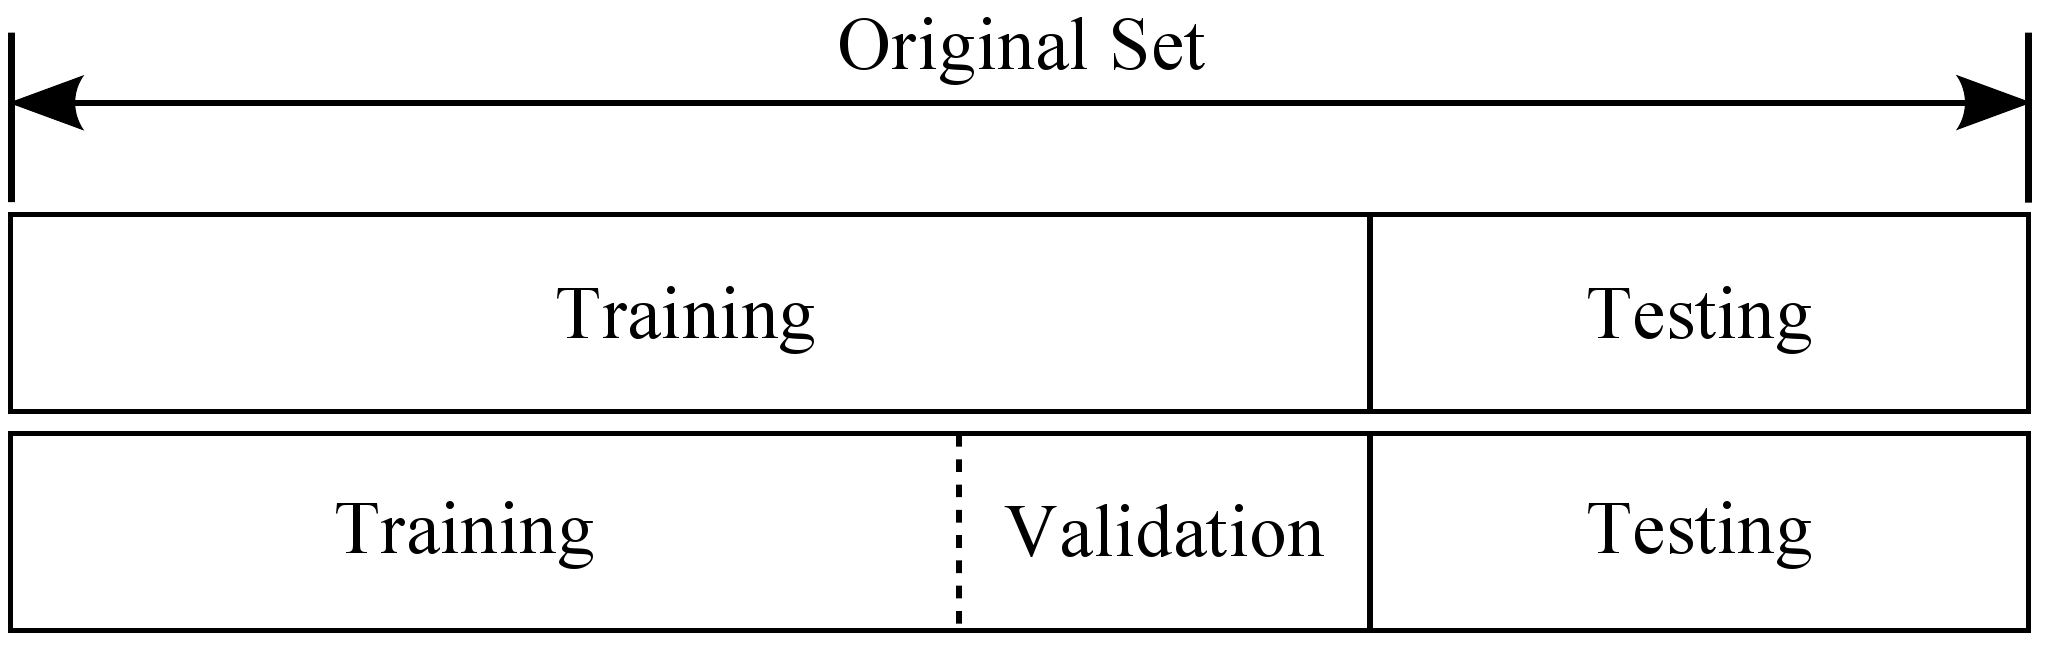
\includegraphics[scale=0.14]{fig3.png}
		\label{fig:fig3}
	\end{figure}

\begin{itemize}
	\item Create similar copula-based arbitrage for triplets to increase information dependency information and measure relative pricing more comprehensively.
	
		\begin{figure}[htbp]
		\centering
		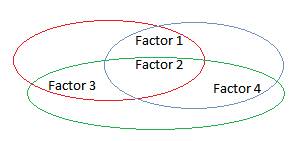
\includegraphics[scale=0.6]{fig4.png}
		\label{fig:fig4}
	\end{figure}
	
	\vspace{0.3cm}
	
	\item Randomized Dependence Coefficient (RDC): measure of nonlinear dependence between random variables of arbitrary dimension. RDC is defined in terms of correlation of random non-linear copula projections (\textcolor{blue}{Lopez-Paz \emph{et al}}., \textcolor{blue}{2013}).
	
\end{itemize}
	
\end{frame}

\begin{frame}[label=frame5b2]
\frametitle{Conclusions}

\begin{enumerate}
	%\setcounter{enumi}{1}
	\justifying
	
\item By capturing linear/nonlinear associations and covering a wider range of possible dependencies structures, the mixed copula strategy is able to generate a higher mean excess return than the distance method when the number of trading signals is equiparable.

\vspace{0.3cm}

\item The alphas of all strategies remain large and significant even after several asset pricing factors such as momentum, liquidity, profitability and investment are taken into account.


\vspace{0.3cm}

\item Future research will focus on the stocks selection process, training/validation/ \newline testing sets and in multidimensional pairs trading to increase dependency information.
	
	
\end{enumerate}

\end{frame}

\begin{frame}
	
	\centering
	\Large{Thanks! Any questions?}
	
\end{frame}

\end{document}







